\documentclass[a4paper,twoside,12pt]{book}
\usepackage{mystyle}

\begin{document}
\parindent 10pt
\pagenumbering{alph}

\title{\Huge\bf \sffamily{Introduction to Automata Theory,\\Formal Languages and \\Computation}}
\author{\Large\bf{Shyamalendu Kandar}\\{Assistant Professor, Computer Science and Engineering}\\ {Haldia Institute of Technology}\\{Haldia, West Bengal}\\{\bf{225 to 228}}}
%\date{%
 % Version~\documentEdition \\
%  \today
%}
\maketitle
\begin{figure}
\centering
 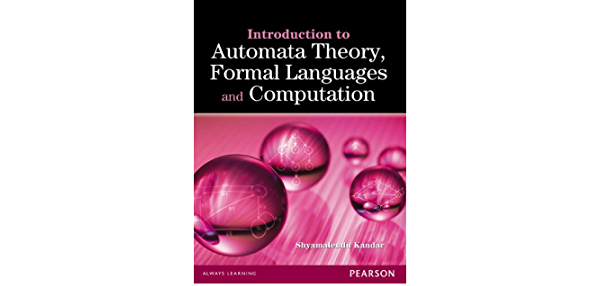
\includegraphics[scale=1]{image/introduction/book}
\end{figure}
%% Copyright page
%{\thispagestyle{empty}
%  \input{tex/notice.tex} \\\\
  %\textbf{Edition} \\
%  Version~\documentEdition \\
%  \today
%}

%% Front matter
%\frontmatter
%\setcounter{tocdepth}{1}
%\tableofcontents
%\let\cleardoublepage\clearpage
%\input{tex/acknowledgments.tex}
%\let\cleardoublepage\clearpage

%% Main document body

\mainmatter
%%%%%%%%%%%%%%%%%%%%%%%%%%%%%%%%%%%%%%%%%%%%
%%%%%%%%%%%%%%%%%%%%%%%%%%%%%%%%%%%%%%%%%%%%%%%% From page 225-228 %%%%%%%%%%%%%%%%%%%%%%%%%%%%%%
\begin{quote}
\footnotesize
%\index{Eulerian trail}
%\index{K\"onigsberg!seven bridges puzzle}
%\index{treasure map}
%\includegraphics[scale=0.7]{image/introduction/konigsberg-treasure-map} \\
%\noindent
%--- Spiked Math,
%\url{http://spikedmath.com/120.html}
\end{quote}
\!\!\!\!\!\!\!\!\!\!\!\!\!\!\!\begin{solution}\\

\noindent\!\!\!\!\!\!\!\!\!\!(i)	The strings that we get from the RE 10*1 are \{11, 101, 1001, 10001…..\}. From the set, we can conclude that the strings that are generated from the REs are beginning with 1 and ending with 1. In between 1 and 1, there are any numbers of 0.\\
\indent So, we can describe in English like this:\\
\indent \emph{Set of all strings beginning and ending with 1 with any number of 0 in between the two 1s.}\\
\indent\!\!\!\!\!\!\!\!\!\!\!\!\!\!\!\!\!(ii)	The strings that we get from the RE a*b* are a* . b*, i.e.,\\

\indent\indent \{Λ, a, aa, aaa, ……\}.\{Λ, b, bb, bbb, …….\}  \{Λ, a, b, aa, bb, ab, abb, aab, ……..\}.\\

\indent From the set, we can conclude that the strings that are generated from the RE contain any num- ber of ‘a’ followed by any number of ‘b’.\\
\indent So, we can describe in English like this:\\

\indent \indent \emph{Set of all strings of ‘a’ and ‘b’ containing any number of ‘a’ followed by any number of ‘b’.}\\

\noindent\!\!\!\!\!\!\!\!\!\!(iii)	The strings that we get from the RE (ab)* are \{Λ, ab, abab, ababab, ………\}.\\
\indent In English, it is described as:\\

\indent \emph{Set of all strings of a and b with equal number of a and b containing ‘ab’ as repetition.}\\

\noindent\!\!\!\!\!\!\!\!\!\!(iv)	(a*  b*) means any combination of a or any combination of b. c* means any combination of c, which is concatenated with (a*  b*).\\
\indent In English, it can be described as:\\

 \indent\emph{Any combination of ‘a’ or any combination of ‘b’ followed by any combination of ‘c’.}\\

\noindent\!\!\!\!\!\!\!\!\!\!(v)	The strings that we get from the RE (00)*(11)*1 are \{1, 001, 111, 00111, ……\}. In the string,\\ there are always odd number of 1 and even number of 0.\\
\indent In English, it can be described as:\\

\indent\indent \emph{Set of all strings of ‘0’ and ‘1’ with even number of 0 followed by odd number of 1.}\\

\noindent Alternatively, the RE described in English language can be denoted using alphabet and symbols. The following examples describe this.\\
\end{solution}
\!\!\!\!\!\!\!\!\!\!\!\!\!\!\!\begin{example}
\textnormal{\small Built regular expression of the following\\
(i)	An RE consists of any combination of a and b, beginning with a and ending with b.\\
(ii)	A language of any combination of a and b containing abb as a substring.\\
(iii)	RE of a and b containing at least 2 ‘a’s.\\
(iv)	Write an RE for the language $L =\{a^nb^m | where m+n is even\}$.\\
(v)	An RE of a and b, having exactly one ‘a’.}
\end{example}

\!\!\!\!\!\!\!\!\!\!\!\!\!\!\!\!\!\!\!\!\begin{solution}

\noindent\!\!\!\!\!\!\!\!\!\!(i)	The RE consists of any combination of a and b, i.e., (a +b)*. But the RE starts with a and ends\\ with b. In between a and b, any combination of a and b occurs. So, the RE is\\
\begin{center}
L = a(a + b)*b.
\end{center}
\end{solution}
%%%%%%%%%%%%%%%%%%%%%%%%%%%%%%%%%%%%%%%%%%%%%% 
\newpage
\begin{quote}
\footnotesize
%\index{Eulerian trail}
%\index{K\"onigsberg!seven bridges puzzle}
%\index{treasure map}
%\includegraphics[scale=0.7]{image/introduction/konigsberg-treasure-map} \\
%\noindent
%--- Spiked Math,
%\url{http://spikedmath.com/120.html}
\end{quote}

\noindent\!\!\!\!\!\!\!\!\!\!(ii)	In the RE, abb occurs as a substring. The RE consists of any combination of a and b. Before the substring, abb may occur at the beginning, at the middle, or at the last. If abb occurs at the begin- ning, then after abb there is any combination of a and b. If abb occurs at the middle, then before and after abb there are any combination of a and b. If abb occurs at the last, then before abb there is any combination of a and b.\\
The RE is L = (a + b)*abb(a +b)*.

\noindent\!\!\!\!\!\!\!\!\!\!(iii)	In the RE, there are at least two ‘a’s. The expression consists of a and b. Therefore, any number of ‘b’
can occur before the first ‘a’ and before the second ‘a’, i.e., after the first ‘a’ and after the second ‘a’. So, the RE will be L = b*ab*ab*.

\noindent\!\!\!\!\!\!\!\!\!\!(iv)	The RE consists of n number of ‘a’ followed by m number of ‘b’. But m +  n is always even. This is possible if\\
(a)	m and n both are even or (b) m and n both are odd.\\
If m and n are both even, then the expression is (aa)*(bb)*.\\ If m and n are both odd, then the expression is (aa)*a(bb)*b.\\ By combining these two, the final RE becomes

\begin{center}
L = (aa)*(bb)* + (aa)*a(bb)*b.
\end{center}
\noindent\!\!\!\!\!\!\!\!\!\!(v)	In the RE, there is exactly one ‘a’. Before and after a, there is any combination of b.\\ Therefore, the RE is L = b*ab*. 

\section{\sffamily{Identities of Regular Expression}}
An \emph{identity} is a relation which is tautologically true. In mathematics, an equation which is true for every value of the variable is called an identity equation. As an example, $(a + b)^2 = a^2 + 2ab + b2$ is an identity equation. Based on these identities, some other problems can be proved. In the RE also, there are some identities which are true for every RE. In this section, we shall discuss those identities related to RE.

\begin{lstlisting}[mathescape=true]
   1.$ \emptyset+R =R+\emptyset =R$

      Proof:$ LHS: \emptyset + R$

             $= \emptyset \cup R$
             $ = \{ \} \cup \{Elements of R\} = R =RHS$
   2. $\emptyset R= R \emptyset =\emptyset$
      Proof:$ LHS: \emptyset R$
              $= \emptyset \cap R$
              $= \{ \} \cap \{Elements of R\} =\emptyset = RHS$

      Note: In both the previous cases, $\emptyset$ denotes a null set, which contains nothing.
   3. $\Lambda R = R\Lambda = R$

      Proof: $LHS: \Lambda R$
              $=$ Null string concatenated with any symbol of R
              $= $Same symbol$ \in R = R = RHS$
   4. $\Lambda* = \Lambda \& \emptyset^* = \Lambda$

      Proof: $LHS: \Lambda^* = \{\Lambda, \Lambda\Lambda, \Lambda\Lambda\Lambda……. \}$
               $=\{\Lambda, \Lambda, \Lambda, …..\} [according to identity (3)]$
               $=\Lambda = RHS.$

      Same for $\emptyset^*$.
\end{lstlisting}
 
%%%%Page Three%%%%%%
\newpage
\begin{quote}
\footnotesize
%\index{Eulerian trail}
%\index{K\"onigsberg!seven bridges puzzle}
%\index{treasure map}
%\includegraphics[scale=0.7]{image/introduction/konigsberg-treasure-map} \\
%\noindent
%--- Spiked Math,
%\url{http://spikedmath.com/120.html}
\end{quote}
\begin{lstlisting}[mathescape=true]
   5. $R+ R = R$

      Proof: $LHS: R + R = R(\Lambda + \Lambda) = R Λ$
              $= R$ [according to identity (3)] $= RHS$

   6. $R^*R^* = R^* $

     Proof: $LHS: R^*R^* = \{\Lambda, R, RR……\} \{\Lambda, R, RR……\}$
               $= \{\Lambda\Lambda, \Lambda R, \Lambda RR, ….., R\Lambda, RR, …, RRΛ, RRR, …. \}$
               $= \{Λ, R, RR, RRR, ….. \} [using identity (3)] = R* = RHS$

   7. $R^*R = RR^*$

     Proof: $LHS: R^*R = \{\Lambda, R, RR, RRR, ….. \} R$
              $ = \{\Lambda R, RR, RRR, RRRR, ….. \}$
               $=  R\{\Lambda, R, RR, RRR, ….. \} = RR^* = RHS$

   8.$ (R^*)^* = R^*$

      Proof:$ LHS: (R^*)^* = \{\Lambda, R^*R^*, R^*R^*R^*, ….. \}$
              $= \{\Lambda, R^*, R^*, ….. \}$ [using identity (6)]
              $= \{\Lambda, \{\Lambda, R, RR, RRR, ….. \}, \{\Lambda, R, RR, RRR, ….. \}, …. \}$
              $=  R^* =  RHS$

   9. $\Lambda + RR^* = \Lambda +  R^*R = R^*$

      Proof: $LHS: \Lambda + RR^* = \Lambda + R \{\Lambda, R, RR, RRR, ….. \}$
             $ = \Lambda + \{R\Lambda, RR, RRR, RRRR, ….. \}$
             $ = \Lambda + \{R, RR, RRR, RRRR, ….. \}$
             $ = \{\Lambda, R, RR, RRR, RRRR, ….. \} = R^* = RHS$

   10. $(PQ)^*P = P(QP)^*$

      Proof: $LHS: (PQ)^*P = \{\Lambda, PQ, PQPQ, PQPQPQ, ….. \}P4
              $= \{P,PQP, PQPQP, PQPQPQP,…..\}4
              $= P\{\Lambda, QP, QPQP, QPQPQP, ……. \}$
              $= P(QP)^* = RHS$

   11. $(P + Q)^* = (P^*Q^*)^* = (P^* + Q^*)^*$ (D’Morgan’s theorem)
   12. $(P + Q)R = PR + QR$

       Proof:$ Let a \in (P+Q)R$
               $= a \in PR or QR = RHS.$
\end{lstlisting}

\!\!\!\!\!\!\!\!\!\!\!\!\!\!\!\begin{example}
\textnormal{\small{From the identities of RE, prove that}}\\

$(1 + 100^*) + (1 + 100^*)(0 + 10^*)(0 + 10^*)^* = 10^*(0  10^*)^*.$
\end{example}
\!\!\!\!\!\!\!\!\!\!\!\!\!\!\!\begin{solution}\small{LHS}.
 \end{solution}
\begin{lstlisting}[mathescape=true]
                        $(1 + 100^*) + (1 + 100^*)(0 + 10^*)(0 + 10^*)^*$
                        $= (1 + 100^*) (\Lambda + (0 + 10^*)(0 + 10^*)^*)$
                        $= (1 + 100^*)(0 + 10^*)^*$ (according to $\Lambda + RR^* = R^*)$
                        $=1(\Lambda + 00^*)(0 + 10^*)^*$
                        $= 10^*(0 + 10^*)^* = RHS.$
\end{lstlisting}

%%%%%%%%%%%%%%%%%%%%%%%%%%%%%%%%%%%%%%%%%%%%%%%%%
\newpage
\begin{example}
\textnormal{\small{From the identities of RE, prove that the following three are equivalent}\\
$(i)\quad(011((11)^* + (01)^*)^*)^*011$\\
$(ii)\quad011(((1 + 0)1)^*011)^*$\\
$(iii)\quad011(((11)^*(01)^*)^*011)^*$}
\end{example}
\!\!\!\!\!\!\!\!\!\!\!\!\!\!\!\begin{solution}\small{Let$ P = (11) and Q =(01).$}
\begin{lstlisting}[mathescape=true]
We know$ (P +Q)^* = (P^*Q^*)^* = (P^* + Q^*)^*.$
Thus, $((11) +(01))^* = ((11)^*(01)^*)^* [in c] =((11)^* +(01)^*)^*[in a] =((1 +0)1)^* [in b].$
 Consider 011 as R and $(P + Q)^*$ as S.
We know that  $(RS)^*R =R(SR)^*$
Thus, $(011((11)^* +(01)^*)^*)^*011 = 011((11)^* + (01)^*)^*011)^*$
                          $= 011((11) + (01))^*011)^*$
                          $= 011(((1 + 0)1)^*011)^*.$
Similarly, $(011((11)* + (01)^*)^*)^*011 = 011((11)^* + (01)^*)^*011)^*$
                               $= 011((11) + (01))^*011)^*$
                               $= 011(((11)^*(01)^*)^*011)^*.$
As $(i) \equiv (ii) and (i) \equiv (iii), (i) \equiv (ii) \equiv (iii).$
\end{lstlisting}
\end{solution}
\begin{example}
\textnormal{\small{From the identities of RE, prove that}
\begin{center}
$10 + (1010)^*[\wedge + (1010)6^*] = 10 + (1010)^*.$
\end{center}}
\end{example}
\!\!\!\!\!\!\!\!\!\!\!\!\!\!\!\begin{solution} \small{LHS $10 + (1010)^*[\wedge + (1010)^*]$}
\begin{lstlisting}[mathescape=true]
           $\Rightarrow10 + \wedge(1010)^* + (1010)^* (1010)^*$
           $\Rightarrow10 + (1010)^*  (1010)^* As \wedge R = R and RR = R$
           $\Rightarrow10 + (1010)^* = RHS. As R + R = R.$
\end{lstlisting}
\end{solution}
\section{\sffamily{The Arden’s Theorem}}
The Arden’s theorem is used to construct the RE from a transitional system of FA.
\setcounter{theorem}{0}
\begin{theorem}\textnormal{
Statement: Let P and Q be two REs over Σ. If P does not contain Λ, then the equation
$R = Q + RP$ has a unique (one and only one) solution, $R = QP^*$.}

\textnormal{
Proof: Now, point out the statements in the Arden’s theorem in general form.
\item{$\square$}{ \textbf P and \textbf Q are two REs}.
\item{$\square$}{ \textbf P does not contain the \textbf Λ symbol.}
\item{$\square$} {\textbf{R =Q + RP} has a solution, i.e., \textbf{R = QP*}.}
\item{$\square$} {This solution is the one and only solution of the equation.}}
\end{theorem}
If R = QP* is a solution of the equation R + Q = RP, then by putting the value of R in the equation, we shall get the value ‘0’.
\begin{lstlisting}[mathescape=true]
                                     $R = Q + RP$
                                     $R - Q - RP = 0$
                                     $ LHS R - Q - RP$
\end{lstlisting}

















%%%%%%%%%%%%%%%%%%%%%%%%%%%%%%%%%%%%%%%%%%%%%%%%

%\input{tex/datastructures.tex}
%\input{tex/trees-forests.tex}
%\input{tex/graph-algorithms.tex}
%\input{tex/graph-data-structures.tex}
%\input{tex/distance-connectivity.tex}
%\input{tex/centrality-prestige.tex}
%\input{tex/optimal-traversals.tex}
%\input{tex/graph-coloring.tex}
%\input{tex/network-flows.tex}
%\input{tex/algebraic-graph-theory.tex}
%\input{tex/random-graphs.tex}
%
%% Appendices
%%%%%\input{tex/license-gfdl.tex}

%% Back matter
%\backmatter
%\cleardoublepage
%\addcontentsline{toc}{chapter}{Bibliography}
%\bibliographystyle{bibliography}
%\bibliography{bibliography}
%\cleardoublepage
%\addcontentsline{toc}{chapter}{Index}
%\printindex

\end{document}